%\documentclass[mathserif]{beamer}
\documentclass[handout]{beamer}
%\usetheme{Goettingen}
\usetheme{Warsaw}
%\usetheme{Singapore}
%\usetheme{Frankfurt}
%\usetheme{Copenhagen}
%\usetheme{Szeged}
%\usetheme{Montpellier}
%\usetheme{CambridgeUS}
%\usecolortheme{}
%\setbeamercovered{transparent}
\usepackage[utf8x]{inputenc} 
\usepackage[spanish]{babel} %idioma
\usepackage{amsmath, amssymb}
\usepackage{dsfont}
\usepackage{graphics}
\usepackage{cases}
\usepackage{graphicx}
\usepackage{pgf}
\usepackage{epsfig}
\usepackage{amssymb}
\usepackage{amstext}
\usepackage[ruled,vlined,lined]{algorithm2e}
\usepackage{amsmath}
\usepackage{epic}
\usepackage{epsfig}
\usepackage{fontenc}
\usepackage{palatino, url, multicol}
%\algsetup{indent=2em}
\newcommand{\factorial}{\ensuremath{\mbox{\sc Factorial}}}
\newcommand{\BIGOP}[1]{\mathop{\mathchoice%
{\raise-0.22em\hbox{\huge $#1$}}%
{\raise-0.05em\hbox{\Large $#1$}}{\hbox{\large $#1$}}{#1}}}
\newcommand{\bigtimes}{\BIGOP{\times}}
\vspace{-0.5cm}
\title{Inferencia Estadística}
\vspace{-0.5cm}
\author[Felipe Bravo Márquez]{\footnotesize
%\author{\footnotesize  
 \textcolor[rgb]{0.00,0.00,1.00}{Felipe José Bravo Márquez}} 

%\vspace{-0.3cm}
%\institute{Universidad de Chile - Departamento de Ciencias de la Computación -Minería de Datos}
\date{ \today }
%\logo{\includegraphics[height=1cm]{imagenes/dcc-small.png}}

\begin{document}
\begin{frame}
\titlepage


\end{frame}


%%%%%%%%%%%%%%%%%%%%%%%%%%%


\begin{frame}{Inferencia Estadística}
\scriptsize{
\begin{itemize}
 \item Para realizar conclusiones sobre una \textbf{población}, generalmente no es factible reunir todos los datos de ésta.
 \item Debemos realizar conclusiones razonables respecto a una población basado en la evidencia otorgada por \textbf{datos muestrales}.
 \item El proceso de realizar conclusiones sobre una población a partir de datos muestrales se conoce como \textbf{inferencia estadística}.
\end{itemize}

} 
\end{frame}


\begin{frame}{Inferencia Estadística (2)}
\scriptsize{
\begin{itemize}
\item En inferencia estadística tratamos de \textbf{inferir} la distribución que genera los datos observados
\item Ejemplo: Dado una muestra $X_1, \dots, X_n \sim F$. ¿Cómo inferimos $F$?
\item En algunos cosas sólo nos interesa inferir alguna propiedad de $F$ como su \textbf{media}.
\item Los modelos estadísticos que asumen que la distribución se puede modelar con un conjunto finito de parámetros $\theta= (\theta_{1},\theta_{2},\dots,\theta_{k})$ se llaman modelos \textbf{paramétricos}.
\item Ejemplo: si asumimos que los datos vienen de una distribución normal $N(\mu,\sigma^2)$, $\mu$ y $\sigma$ serían los parámetros del modelo. 
\item Un \textbf{estadístico} (muestral) es una medida cuantitativa calculada a partir de los datos.
\end{itemize}


} 
\end{frame}




\begin{frame}{Estimación Puntual}
\scriptsize{
\begin{itemize}
 \item La estimación puntual es el proceso de encontrar la \textbf{mejor aproximación} de una cantidad de interés a partir de una \textbf{muestra estadística}.
 \item La cantidad de interés puede ser: un parámetro en un modelo paramétrico, una CDF, una PDF, o una función de regresión.
 \item Por convención se denota a la estimación puntual del valor de interés $\theta$ como $\hat{\theta}$ o $\hat{\theta}_n$ 
 \item Es importante remarcar que mientras $\theta$ es un valor fijo desconocido, $\hat{\theta}$  depende de los datos y por ende es una variable aleatoria. 

\end{itemize}

} 
\end{frame}

\begin{frame}{Estimación Puntual (2)}

\scriptsize{
\begin{block}{Definición Formal}
\begin{itemize}
 \item Sean $X_1, \dots, X_n$ $n$ observaciones IID de una distribución $F$
 \item Un estimador puntual $\hat{\theta}_n$  de un parámetro $\theta$ es una función de $X_1, \dots, X_n$:
 \begin{displaymath}
 \hat{\theta}_n=g(X_1, \dots, X_n) 
 \end{displaymath}
 
\end{itemize}

 
\end{block}

\begin{itemize}
 \item El \textbf{sesgo} (bias) de un estimador se define como: 
\begin{displaymath}
 \text{bias}(\hat{\theta}_n)=\mathbb{E}(\hat{\theta}_n)-\theta
\end{displaymath}
\item Un estimador es insesgado si $\mathbb{E}(\hat{\theta}_n)=\theta$ o  $\text{bias}(\hat{\theta}_n)=0 $
\end{itemize}

} 
\end{frame}


\begin{frame}{Estimación Puntual (3)}

\scriptsize{

\begin{itemize}
\item La distribución de $\hat{\theta}_n$ se conoce como la \textbf{distribución muestral}
\item La desviación estándar de $\hat{\theta}_n$ se conoce como \textbf{error estándar} $se$:
\begin{displaymath}
se(\hat{\theta}_n)=\sqrt{\mathbb{V}(\hat{\theta}_n})
\end{displaymath}
\item El error estándar nos habla sobre la variabilidad del estimador entre todas las posibles muestras de un mismo tamaño.
\end{itemize}

} 
\end{frame}


\begin{frame}{Estimación Puntual (4)}
\scriptsize{

\begin{itemize}
 \item Sea $X_1,X_2,\dots,X_n$ una muestra aleatoria de una población de media $\mu$ y varianza $\sigma^2$
 \item Se define la \textbf{media muestral} $\overline{X_{n}}$ o $\hat{\mu}$ como:
 \begin{displaymath}
  \overline{X_{n}}=\frac{1}{n}\sum_{i=1}^{n} X_i
 \end{displaymath}
\item Es un estimador insesgado:
\begin{displaymath}
\mathbb{E}(\overline{X_{n}}) = \mathbb{E}(\frac 1n \sum_{i=1}^{n} X_i)  =  \frac 1n \times \mathbb{E}(\sum_{i=1}^{n} X_i) = \frac 1n (n \times \mu) = \mu  
\end{displaymath}

\item Su error estándar sería $se(\overline{X_{n}}) = \sqrt{\mathbb{V}(\overline{X_{n}})}$ donde
\begin{displaymath}
 \mathbb{V}(\overline{X_{n}})=\mathbb{V}(\frac 1n \sum_{i=1}^{n} X_i) = \frac{1}{n^2} \mathbb{V}(\sum_{i=1}^{n} X_i) = \frac{n}{n^2} \mathbb{V}(X_i)=\frac{\sigma^2}{n} 
\end{displaymath}

\item Entonces $se(\overline{X_{n}}) = \frac{\sigma}{\sqrt{n}}$

\end{itemize}


} 
\end{frame}


\begin{frame}{Ejemplos de Estimación Puntual (5)}
\scriptsize{
\begin{itemize}
 \item Por lo general no sabemos $\sigma$ de la población.
 \item Cuando queremos estimar la varianza de una población a partir de una muestra hablamos de la  \textbf{varianza muestral}:
\item Existen dos estimadores comunes, una versión sesgada \begin{displaymath}
 s_{n}^{2}= \frac{1}{n} \sum_{i}^{n}(X_{i}-\overline{X_{n}})^2
\end{displaymath}

\item Una versión sin sesgo \begin{displaymath}
 s^{2}= \frac{1}{n-1} \sum_{i}^{n}(X_{i}-\overline{X_{n}})^2
\end{displaymath}

\item Cuando no sabemos la varianza de la población y queremos estimar la media, el error estándar es estimado: \begin{displaymath}                                                                                                                 
\hat{se}(\overline{X_{n}}) = \frac{s}{\sqrt{n}}                                                                                                                \end{displaymath}


\end{itemize}


} 
\end{frame}


\begin{frame}{Estimación Puntual (6)}
\scriptsize{
\begin{itemize}
 \item Sean $X_1, \dots, X_n \sim$ Bernoulli$(p)$ y sea $\hat{p}_{n}=\frac 1n \sum_{i}X_{i}$
 \item Luego $\mathbb{E}(\hat{p}_{n})= \frac 1n \sum_i \mathbb{E}(X_i)=p$, entonces $\hat{p}_n$ es insesgado.
 \item El error estándar $se$ sería
\begin{displaymath}
se = \sqrt{\mathbb{V}(\hat{p}_n)}= \sqrt{p(1-p)/n} 
\end{displaymath}
\item El error estándar estimado $\hat{se}$:
\begin{displaymath}
\hat{se} =\sqrt{\hat{p}(1-\hat p)/n} 
\end{displaymath}

\end{itemize}


} 
\end{frame}




\begin{frame}{Estimación Puntual (7)}

\scriptsize{

\begin{itemize}
\item Se espera que un buen estimador sea insesgado y de mínima varianza.
\item Un estimador puntual $\hat{\theta}_n$ de un parámetro $\theta$ es \textbf{consistente} si converge al valor verdadero cuando el número de datos de la muestra tiende a infinito.
\item La calidad de un estimador se puede medir usando el \textbf{error cuadrático medio} (MSE)
\begin{displaymath}
MSE = \mathbb{E}_{\theta}(\hat{\theta}_n - \theta)^2 
\end{displaymath}

\end{itemize}

} 
\end{frame}



\begin{frame}{Estimación Puntual (8)}

\scriptsize{

\begin{itemize}
\item Si para un estimador $\hat{\theta}_n$, su $bias \rightarrow 0$ y su $se \rightarrow 0$ cuando $n\rightarrow \infty$, $\hat{\theta}_n$ es un estimador consistente de $\theta$.

\item Por ejemplo, para la media muestral $\mathbb{E}(\overline{X_{n}})=\mu$ lo que implica que el $bias =0$ y $se(\overline{X_{n}}) = \frac{\sigma}{\sqrt{n}}$ que tiende a cero cuando $n\rightarrow \infty$. Entonces $\overline{X_{n}}$ es un estimador consistente de la media.  

\item Para el caso del experimento Bernoulli se tiene que $\mathbb{E}(\hat{p})=p \Rightarrow bias=0$ y $se = \sqrt{p(1-p)/n} \rightarrow 0$ cuando $n\rightarrow \infty$. Entonces $\hat{p}$ es un estimador consistente de $p$.


\end{itemize}

} 
\end{frame}



\begin{frame}{Intervalo de Confianza}
\scriptsize{
\begin{itemize}
 \item Sabemos que el valor de un estimador puntual \textbf{varía} entre una muestra y otra
 \item Es más razonable encontrar un \textbf{intervalo} donde sepamos que valor \textbf{real del parámetro} se encuentra dentro del intervalo con una cierta \textbf{probabilidad}.
 \item La forma general de un intervalo de confianza en las siguiente:
  \begin{displaymath}
   \text{Intervalo de Confianza} = \text{Estadístico Muestral} \ \pm \ \text{Margen de Error}
  \end{displaymath}
 \item Entre más ancho el intervalo mayor incertidumbre existe sobre el valor del parámetro.
\end{itemize}


}
 
\end{frame}


\begin{frame}{Intervalo de Confianza (2)}
\scriptsize{

\begin{block}{Definición}
\begin{itemize}
 \item Un \textbf{intervalo de confianza} para un parámetro poblacional desconocido $\theta$ con un \textbf{nivel de confianza} $1-\alpha$, es un intervalo $C_n = (a,b)$ donde:
\begin{displaymath}
 \mathbb{P}(\theta \in C_n) = 1-\alpha
\end{displaymath}
 \item Además $a= a(X_1, \dots, X_n)$ y $b=b(X_1,\dots,X_n)$ son funciones de los datos
 \item El valor $\alpha$ se conoce como el nivel de \textbf{significancia}, generalmente se toma como $0.05$ lo que equivale a trabajar con un nivel de confianza de $95\%$
 \item La significancia se puede interpretar como la probabilidad de equivocarnos.
\end{itemize}

\end{block}

}
 
\end{frame}


\begin{frame}{Intervalo de Confianza (3)}
\scriptsize{

\begin{block}{Interpretación}
\begin{itemize}
 \item Existe mucha \textbf{confusión} de como interpretar un intervalo de confianza
 \item Una forma de interpretarlos es decir que si repetimos \textbf{un mismo experimento} muchas veces, el intervalo contendrá el valor del parámetro el $(1-\alpha)\%$ de las veces.
 \item Esta interpretación es correcta, pero rara vez repetimos un mismo experimento varias veces.
 \item Una interpretación mejor: un día recolecto datos creo un intervalo de $95\%$ de confianza para un parámetro $\theta_1$. Luego, en el día 2 hago lo mismo para un parámetro $\theta_2$ y así reiteradamente $n$ veces. El $95\%$ de mis intervalos \textbf{contendrá} los valores reales de los parámetros.
 
\end{itemize}

\end{block}

}
 
\end{frame}

\begin{frame}{Intervalo de Confianza (4)}
\scriptsize{
\begin{itemize}
 \item Se tienen $n$ observaciones independientes $X_1, \dots, X_n$ IID de distribución  $N(\mu,\sigma^2)$
 \item Supongamos que $\mu$ es \textbf{desconocido} pero $\sigma^2$ es \textbf{conocido}.
 \item Sabemos que $\overline{X_{n}}$ es un estimador insesgado de $\mu$
 \item Por la ley de los grandes números sabemos que la distribución de $\overline{X_{n}}$ se concentra alrededor de $\mu$ cuando $n$ es grande.
 \item Por el CLT sabemos que \begin{displaymath}
 Z=\frac{\overline{X_{n}}-\mu}{\frac{\sigma}{\sqrt{n}}}  \sim N(0,1)
\end{displaymath}
cuando $n$ es grande
\item Despejando, tenemos que $\mu = \overline{X_{n}} - \frac{\sigma}{\sqrt{n}}Z$
\end{itemize}


 }
\end{frame}

\begin{frame}{Intervalo de Confianza (5)}
\scriptsize{
\begin{itemize}
 \item Queremos encontrar un intervalo intervalo $C_n = (\mu_1,\mu_2)$ con un nivel de confianza $1-\alpha$:
\begin{displaymath}
 \mathbb{P}(\mu_1 \leq \mu \leq \mu_2 ) = 1-\alpha
\end{displaymath}
\item Sea $z_a = \Phi^{-1}(1-a)$, con $a \in [0,1]$ donde $\Phi^{-1}$ es la función cuantía de una normal estandarizada
\item Esto es equivalente a decir que $z_a$ es el valor tal que $1-\Phi(z_a)=\mathbb{P}(Z \geq z_a)=a$

\item Por simetría de la normal $z_{\alpha/2}=-z_{(1-\alpha/2)}$
\end{itemize}


 }
\end{frame}



\begin{frame}{Intervalo de Confianza (6)}
\scriptsize{
\begin{itemize}
 \item Se tiene que \begin{displaymath}
\mathbb{P}(-z_{\alpha/2}<Z<z_{\alpha/2})=1-\alpha                     
                    \end{displaymath}

\begin{figure}[h!]
	\centering
	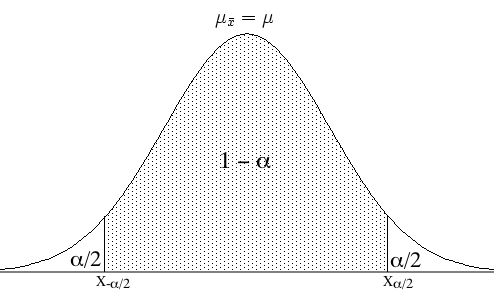
\includegraphics[scale=0.35]{imagenes/ConfIntervNormalP.png}
\end{figure}




\end{itemize}
}
 
\end{frame}

\begin{frame}{Intervalo de Confianza (7)}
\scriptsize{
\begin{itemize}
 \item  El intervalo de confianza para $\mu$ es:
 \begin{displaymath}
 C_n = (\overline{X_{n}}-z_{\alpha/2}\frac{\sigma}{\sqrt{n}} , \overline{X_{n}} + z_{\alpha/2}\frac{\sigma}{\sqrt{n}}) 
 \end{displaymath}
\item Entonces $ z_{\alpha/2}$ nos dice cuantas veces tenemos que multiplicar el \textbf{error estándar} en el intervalo.
\item Mientras menor sea $\alpha$ mayor será $ z_{\alpha/2}$ y por ende más ancho será el intervalo. 
\item Demostración:
 \begin{eqnarray*}
 \mathbb{P}(\mu \in C_n) & = & \mathbb{P}(\overline{X_{n}}-z_{\alpha/2}\frac{\sigma}{\sqrt{n}} < \mu < \overline{X_{n}} + z_{\alpha/2}\frac{\sigma}{\sqrt{n}}) \nonumber \\ 
                         & = & \mathbb{P}(-z_{\alpha/2} < \frac{\overline{X_{n}}-\mu}{\frac{\sigma}{\sqrt{n}}} <  z_{\alpha/2}) \nonumber \\ 
			  & = & \mathbb{P}(-z_{\alpha/2} < Z <  z_{\alpha/2}) \nonumber \\
			   & = & 1-\alpha 
 \end{eqnarray*}


\end{itemize}
}


 
\end{frame}

\begin{frame}[fragile]{Intervalo de Confianza (8) }

\scriptsize{
\begin{itemize}
 \item Como $z_{\alpha/2} = \Phi^{-1}(1-\alpha/2)$ podemos usar la función cuantía de la normal para calcular intervalos de confianza en R
\end{itemize}


\begin{verbatim}
> alpha <- 0.05
> xbar <- 5
> sigma <- 2
> n <- 20
> se <-sigma/sqrt(n)
> error <- qnorm(1-alpha/2)*se
> left <- xbar-error
> right <- xbar+error
> left
[1] 4.123477
> right
[1] 5.876523
>
\end{verbatim}
}



\end{frame}

\begin{frame}{Distribución T}
\scriptsize{
\begin{itemize}
 \item En la pŕactica, si no conocemos $\mu$ es poco probable que conozcamos $\sigma$
 \item Si estimamos $\sigma$ usando $s$, los intervalos de confianza se construyen usando la distribución \textbf{T-student}
\end{itemize}

\begin{block}{Distribución T}
\begin{itemize}
 \item Una V.A tiene distribución $t$ con $k$ grados de libertad cuando tiene la siguiente PDF:
\begin{displaymath}
 f(t)=\frac{\Gamma(\frac{k+1}{2})}{\sqrt{k\pi}\Gamma(\frac k2)(1+\frac{t^2}{k})^{(k+1)/2}}
\end{displaymath}
\item Cuando $k=1$ se le llama distribución de \textbf{Cauchy}
\item Cuando $k\rightarrow \infty$ converge a una distribución normal estandarizada
 \item La distribución t tiene colas más anchas que la normal cuando tiene pocos grados de libertad


\end{itemize}

 
\end{block}




} 
\end{frame}

\begin{frame}[fragile]{Distribución T (2)}
 \scriptsize{



\begin{verbatim*}
x<-seq(-8,8,length=400)
y1<-dnorm(x)
y2<-dt(x=x,df=1)
y3<-dt(x=x,df=10)
y4<-dt(x=x,df=350)
plot(y1~x,type="l",col="green")
lines(y2~x,type="l",col="blue")
lines(y3~x,type="l",col="black")
lines(y4~x,type="l",col="red")

\end{verbatim*}

 \begin{figure}[h!]
	\centering
	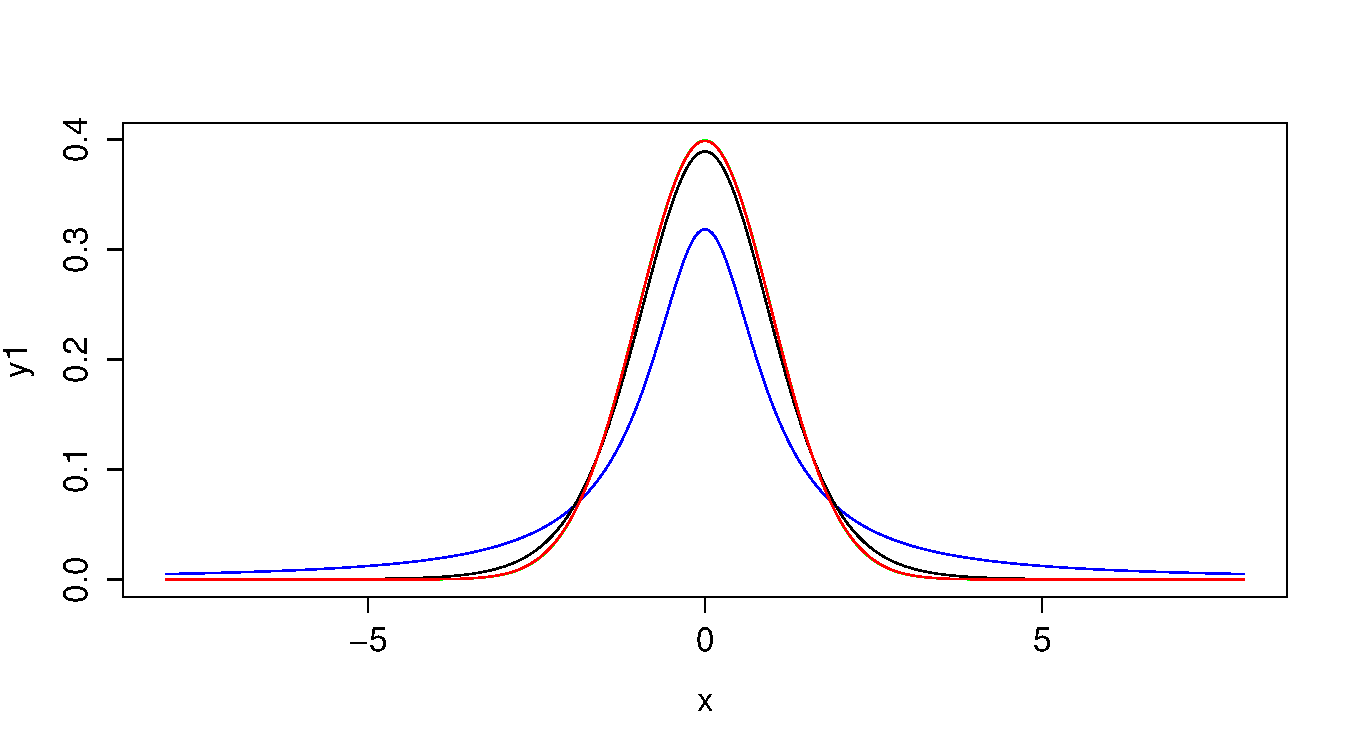
\includegraphics[scale=0.3]{imagenes/tstudent.pdf}
\end{figure}


}
\end{frame}


\begin{frame}{Intervalo de Confianza (9) }

\scriptsize{
\begin{itemize}
 \item Sea  $s^{2}= \frac{1}{n-1} \sum_{i}^{n}(X_{i}-\overline{X_{n}})^2$ tenemos:
 \begin{displaymath}
  T=\frac{\overline{X_{n}}-\mu}{\frac{s}{\sqrt{n}}}\sim t_{n-1}
 \end{displaymath}
\item Sea $t_{n-1,a}=\mathbb{P}(T>a)$, equivalente a la función cuantía $qt$ evaluada en $(1-a)$
\item El intervalo de confianza resultante es:
       \begin{displaymath}
 C_n = (\overline{X_{n}}-t_{n-1,\alpha/2}\frac{s}{\sqrt{n}} , \overline{X_{n}} + t_{n-1,\alpha/2}\frac{s}{\sqrt{n}}) 
 \end{displaymath} 
 \item Como las colas de la distribución $t$ son más anchos cuando $n$ es pequeño, los intervalos de confianza resultantes son más anchos

\end{itemize}


}

\end{frame}


\begin{frame}[fragile]{Intervalo de Confianza (10)}
\scriptsize{
\begin{itemize}
 \item Calculemos un intervalo de confianza para la media de \verb+Petal.Length+ de los datos del \textbf{Iris} con $95\%$ de confianza
\begin{verbatim}
>data(iris)
>alpha<-0.05
>n<-length(iris$Petal.Length)
>xbar<-mean(iris$Petal.Length)
>xbar
[1] 3.758
>s<-sd(iris$Petal.Length)
>se<-s/sqrt(n)
>error<-qt(p=1-alpha/2,df=n-1)*se
>left<-xbar-error
>left
[1] 3.473185
>right<-xbar+error
>right
[1] 4.042815
\end{verbatim}
\item Otra forma:
\begin{verbatim}
>test<-t.test(iris$Petal.Length,conf.level=0.95)
>test$conf.int
[1] 3.473185 4.042815
\end{verbatim}


\end{itemize}



}
 
\end{frame}

\begin{frame}{Test de Hipótesis}
\scriptsize{
\begin{itemize}
 \item Cuando queremos probar si alguna \textbf{propiedad} asumida sobre una población se contrasta con una muestra estadística usamos un \textbf{Test de Hipótesis}
\item El test se compone de las siguientes hipótesis:
 \begin{itemize}
\scriptsize{
\item \textbf{Hipótesis Nula} $H_{0}$: Simboliza la situación actual. Lo que se ha considerado real hasta el presente.
\item \textbf{Hipótesis Alternativa} $H_{a}$: es el modelo alternativo que queremos considerar. 
}
 \end{itemize}
\item La idea es encontrar suficiente \textbf{evidencia estadística} para rechazar $H_{0}$ y poder concluir $H_{a}$
\item Si no tenemos suficiente evidencia estadística \textbf{fallamos en rechazar} $H_{0}$

\end{itemize}



} 
\end{frame}



\begin{frame}{Test de Hipótesis (2)}
\scriptsize{

\begin{block}{Metodología para Realizar un Test de Hipótesis}
\begin{itemize}
 \item Elegir una hipótesis nula $H_0$ y alternativa $H_a$
 \item Fijar un nivel de significancia $\alpha$ del test
 \item Calcular un estadístico $T$ a partir de los datos
 \item El estadístico $T$ es generalmente un valor estandarizado que podemos chequear en una tabla de distribución
 \item Definir un criterio de rechazo para la hipótesis nula. Generalmente es un valor crítico $c$.
\end{itemize}
\end{block}



} 
\end{frame}



\begin{frame}[fragile]{Test de Hipótesis (3)}
\scriptsize{
\begin{itemize}
 \item Ejemplo: Se sabe que la cantidad de horas promedio de uso de Internet mensual en Chile país es de 30 horas
 \item Supongamos que queremos demostrar que el promedio es distinto a ese valor.
 \item Tendríamos que $H_0: \mu=30$ y $H_{a}: \mu \neq 30$
 \item Fijamos $\alpha=0.05$ y recolectamos 100 observaciones
 \item Supongamos que obtenemos $\overline{X_{n}}=28$ y $s=10$
 \item Una forma de hacer el test es construir un intervalo de confianza para $\mu$ y ver si $H_{0}$ está en el intervalo.
\begin{verbatim}
> 28-qt(p=0.975,99)*10/sqrt(100)
[1] 26.01578
> 28+qt(p=0.975,99)*10/sqrt(100)
[1] 29.98422 
\end{verbatim}
\item El intervalo sería la zona de aceptación de $H_0$ y todo lo que esté fuera de éste será mi región de rechazo.
\item Como 30 está en la región de rechazo, rechazo mi hipótesis nula con un $5\%$ de confianza.
\end{itemize}



} 
\end{frame}


\begin{frame}[fragile]{Test de Hipótesis (4)}
\scriptsize{
\begin{itemize}
 \item Otra forma de realizar el test es calcular el estadístico $T=\frac{\overline{X_{n}}-\mu_{o}}{\frac{s}{\sqrt{n}}}$
 \item En este caso sería \begin{displaymath}
                           T=\frac{28-30}{\frac{10}{\sqrt{100}}}=-2
                          \end{displaymath}
\item Como $H_{a}: \mu \neq 30$, tenemos un test de dos lados, donde la región de aceptación es
\begin{displaymath}
 t_{n-1,1-\alpha/2}<T<t_{n-1,\alpha/2}
\end{displaymath}
\begin{verbatim}
 > qt(0.025,99)
[1] -1.984217
> qt(0.975,99)
[1] 1.984217
\end{verbatim}
\item Como $T$ está en la región de rechazo, rechazamos la hipótesis nula.

\end{itemize}



} 
\end{frame}


\begin{frame}[fragile]{Test de Hipótesis (5)}
\scriptsize{
\begin{itemize}
 \item Generalmente, además de saber si rechazamos o fallamos en rechazar una hipótesis nula queremos saber la evidencia que tenemos en contra de ella.
 \item Se define un \textbf{p-valor} como la probabilidad de obtener un resultado al menos tan extremo como el observado en los datos dado que la hipótesis nula es verdadera.
 \item ``Extremo'' significa lejos de la hipótesis nula.
 \item Si el \textbf{p-valor} es menor que el nivel de significancia $\alpha$, rechazamos $H_{0}$ 
 \item Ejemplo:
\begin{verbatim}
> data(iris)
> mu<-3 # La hipótesis nula
> alpha<-0.05
> n<-length(iris$Petal.Length)
> xbar<-mean(iris$Petal.Length)
> s<-sd(iris$Petal.Length)
> se<-s/sqrt(n)
> t<-(xbar-mu)/(s/sqrt(n))
> pvalue<-2*pt(-abs(t),df=n-1)
> pvalue
[1] 4.94568e-07 # es menor que 0.05 entonces rechazamos H0
\end{verbatim}
\end{itemize}

 


}
\end{frame}

\begin{frame}[fragile]{Test de Hipótesis (6)}
\scriptsize{
\begin{itemize}
 \item La forma elegante de hacerlo en R:
\end{itemize}

\begin{verbatim}
> t.test(x=iris$Petal.Length,mu=3)

	One Sample t-test

data:  iris$Petal.Length 
t = 5.2589, df = 149, p-value = 4.946e-07
alternative hypothesis: true mean is not equal to 3 
95 percent confidence interval:
 3.473185 4.042815 
sample estimates:
mean of x 
    3.758 
\end{verbatim}
}



\end{frame}

\begin{frame}{Test de Hipótesis (7)}
 \scriptsize{

\begin{itemize}
 \item Tenemos dos tipos de errores cuando realizamos un test de hipótesis
 \item Error tipo I: es cuando rechazamos la hipótesis nula cuando ésta es cierta.
 \item Este error es equivalente al nivel de significancia $\alpha$
 \item Error tipo II: es cuando la hipótesis nula es falsa pero no tenemos evidencia estadística para rechazarla.
 \item Para mitigar los errores tipo I generalmente usamos valores de $\alpha$ más pequeños.
 \item Para mitigar los errores tipo II generalmente trabajamos con muestras más grandes.
 \item Existe un trade-off entre los errores tipo I y tipo II. 
\end{itemize}

 \begin{table}
\begin{tabular}{c | c c}
\hline
  & Retener $H_0$ &  Rechazar $H_{0}$   \\ 
\hline
$H_0$ es verdadera & \checkmark & error tipo I \\
$H_1$ es verdadera & error tipo II & \checkmark \\
\hline
\end{tabular}
\end{table}

}
\end{frame}





%%%%%%%%%%%%%%%%%%%%%%%%%%%
\begin{frame}[allowframebreaks]\scriptsize
\frametitle{Bilbiografía}
%\bibliography{bio}
%\bibliographystyle{apalike}
\begin{thebibliography}{8}

\bibitem{Assaad2008}
L. Wasserman \emph{All of Statistics: A Concise Course in Statistical Inference}, Springer Texts in Statistics, 2005.
\end{thebibliography}

%\bibliographystyle{flexbib}
\end{frame}









%%%%%%%%%%%%%%%%%%%%%%%%%%%

\end{document}
